\section{Use Cases}
The three proposed visualizations are evaluated by presenting an exemplary use case each visualization helps to solve, based on the questions we identified in Table~\ref{table-questions} in Section~\ref{visualizations}.

\subsection{Seasonality in the Paris Region}
\begin{figure}
    \centering
    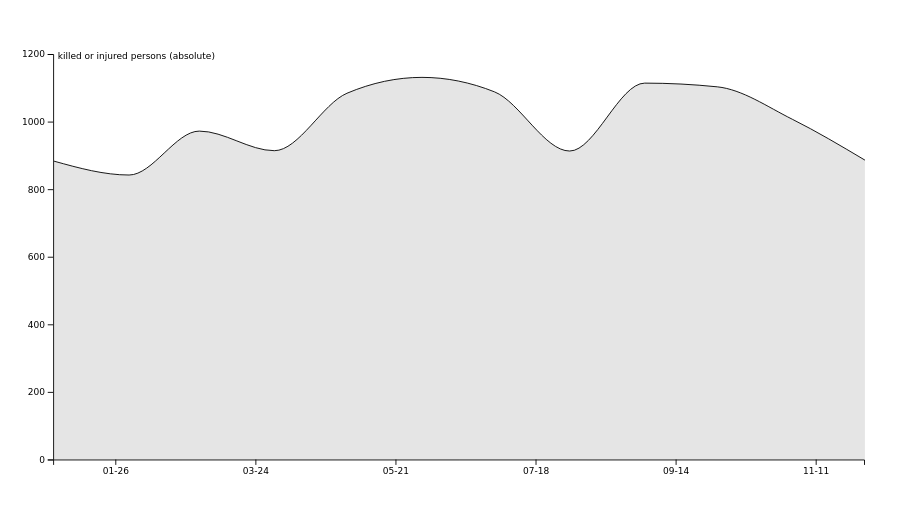
\includegraphics[width=0.9\linewidth]{figures/time-series-2-to-1-killed-or-injured-absolute-by-year-per-month.png}
    \caption{Time series of the number of killed or injured persons per month with a 2:1~aspect ratio, by aggregating across all years~2005--2010.}
    \label{figure-time-series-killed-injured-by-year-per-month}
\end{figure}
An interesting use case for the time series plot is to answer the question whether there is a seasonal influence on the prevalence and severity of road accidents. A citizen living in Paris might ask the following: \enquote{Are roads more dangerous in winter or summer?}
By aggregating injured or killed persons across recent years~(2005--2020) and grouping per month, we get the time series visualization in Figure~\ref{figure-time-series-killed-injured-by-year-per-month}. To be able to spot seasonal trends, we also enable banking to 45\(^\circ\). First, we observe that the monthly number of injured or killed persons is above~800 for all months. But even though one could intuitively think driving in winter would be more dangerous, from December to March there are fewer road casualties.
Because the citizen lives in Paris, they would like to check whether the findings also hold true when only considering accidents from the Paris metropolitan area.
Therefore they switch to the map view to select a grouping by Departements and click on their Departement of Paris. 
With our current implementation this use case faces two difficulties: \Ni because Paris is divided into several Departements, it can be difficult to select the correct Departement from the map and \Nii becuase of the sampling described in Section~\ref{data} the selected sub-set is to small to observe any trends in the time series plot.
In future work, we plan to improve this interaction by optimizing the application code to work with the whole dataset.
Arguably the citizen could also find this seasonal influence in a recursive pattern visualization. But the color mapping of the recursive pattern technique would make it difficult, especially for color-blind people, to distinguish and quantify the extent of seasonality.

\subsection{Prevalence of Woman}
\begin{figure}
    \centering
    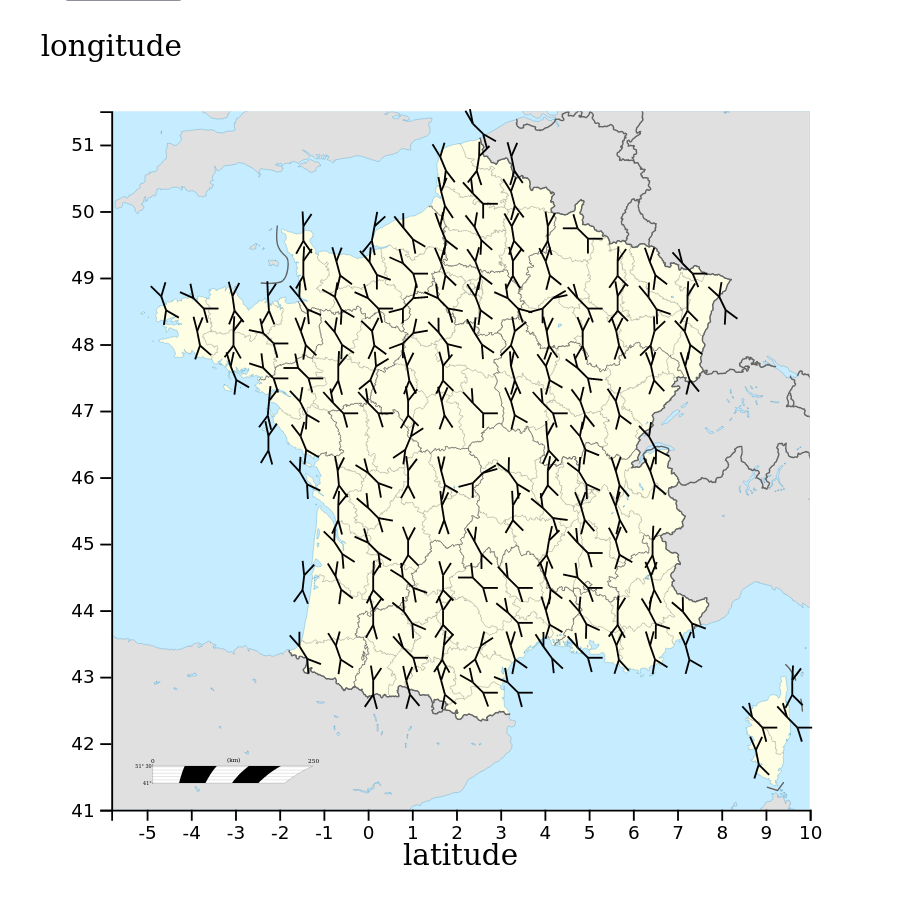
\includegraphics[width=0.6\linewidth]{figures/stick-figures-by-grid-20-20-average.png}
    \caption{Stick figure icons of average person characteristics on a map of France after partitioning the map into a \(20 \times 20\)~grid.}
    \label{figure-stick-figures-grid-average}
\end{figure}
For the second use case, a policy maker would like to answer the question: \enquote{Do women drive more carefully?} They would also like to know if that is true for specific regions in France.
To answer this information need, they open the person characteristics map and select a grouping by a \(20 \times 20\)~grid as shown in Figure~\ref{figure-stick-figures-grid-average}.
Features are aggregated by averaging across the individual persons in each of the 400~grid cells. The resulting stick figures indicate that for most regions in France the majority of participants in road accidents is male, thereby confirming the policy maker's question.
Interestingly however, in some regions there are equally many accidents involving men as there are involving women, especially in coastal regions.
In contrast to other visualization techniques such as Chernoff faces, the stick figures induce a texture on the map, where the rotated figures are visible as a \enquote{flow} from north-west to south-east.
However, other icon-based techniques might work better to emphasize differences in the other 4~plotted dimensions, because with stick figures smaller differences only result in barely noticable angular changes in the stick figure.
In our visualization application this limitation can be avoided by selecting the x-ray stick figure style as then the individual stick figures differ more than with averaging, resulting in greater differences of the stick figure angles.

\subsection{Rainy Nights}
\begin{figure}
    \centering
    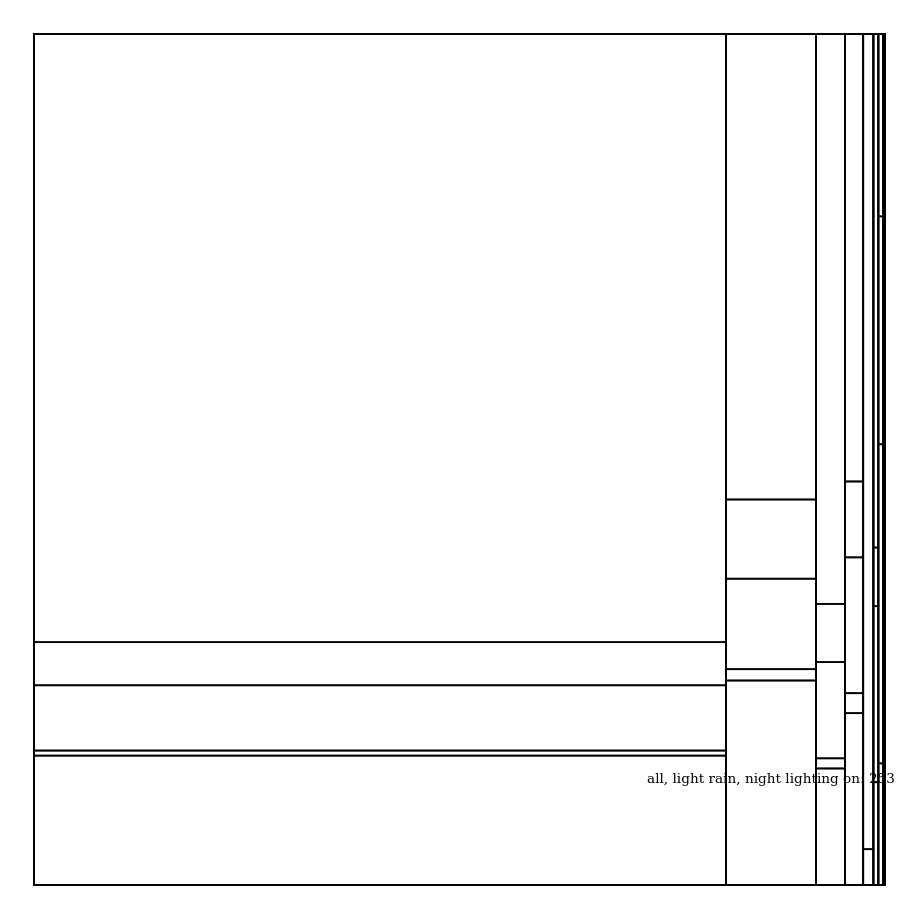
\includegraphics[width=0.6\linewidth]{figures/tree-treemap-weather-light-condition.png}
    \caption{Tree map of accidents by weather and light condition.}
    \label{figure-treemap-weather-light-condition}
\end{figure}
Our last use case is a public infrastudture planner wondering where the current infrastrucure might not suffice in mitigating road accidents. Because they are aware that the majority of accidents occurs under normal conditions~(i.e., with normal weather and in daylight), they would like to identify unexpectedly high numbers of accidents, specifically targetting the public lighting.
This use case is relevant because after decades of development in public infrastructure planning, good starting points for infrastructure projects are not always obvious to find. 
In the treemap visualization they therefore select the weather dimension followed by the light condition dimension.
The resulting treemap is shown in Figure~\ref{figure-treemap-weather-light-condition} and indicates that indeed the majority~(5769~accidents) occur in daylight when the weather conditions are normal.
However, by comparing the number of accidents with public lighting enabled, the treemap indicates that when it rains disproportionately many accidents occur with enabled public lighting. Hence, it would make sense to investigate whether the lights are either too dimmed, leading to limited visibility, or too bright, blinding drivers that pass public lighting.
Even though in this case only three dimensions~(weather, light condition, number of accidents) are visualized, the treemap visualizaiton is still inferior to a scatterplot, because in a scatterplot the number of accidents~(clusters of points in the plot) would not be as easy to interpret as with a treemap node's area.
